\section{ЗАДАНИЕ}

Разработать своюю программу <<Телефонный справочник>>. Протестировать работу программы. Добиться того, чтобы в результате выполнения текстовой программы возращалось несколько вариантов ответов.

\begin{lstlisting}[caption=Текст программы]
domains
	firstname, lastname = string.
	telephone = integer.
predicates
	note(firstname, lastname, telephone).
clauses
	note("Ivan", "Ivanov", 111111111).
	note("Ivan", "Smirnov", 123456789).
	note("Petr", "Petrov", 222222222).
	note("Vasilii", "Vasiliev", 333333333).
goal
	note("Ivan", Lastname, Telephone).
\end{lstlisting}

\begin{figure}[H]
    \centering
    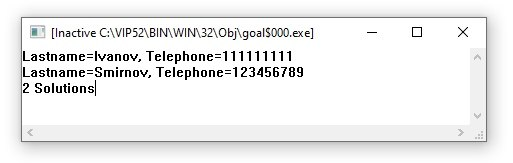
\includegraphics{img/result.jpg}
    \caption{Результат работы программы}
\end{figure}

\section{ПРОГРАММА НА PROLOG}

С помощью термов, фактов и правил <<описываются>> знания о предметной области, то есть \textbf{база знаний}. Используя базу знаний, система Prolog будет делать логические выводы, отвечая на наши вопросы. Таким образом, \textbf{программа на Prolog представляет собой базу знаний и вопрос}.

\subsection{Структура программы}

\begin{itemize}
    \item директивы компилятора -- зарезервирвоанные символьные константы
    \item CONSTANST -- раздел описания констант
    \item DOMAINS -- раздел описания доменов
    \item DATABASE -- раздел описания предикатов внутренней базы данных
    \item PREDICATES -- раздел описания предикатов
    \item CLAUSES -- раздел описания предложений базы знаний
    \item GOAL -- раздел описания внутренней цели (вопроса)
\end{itemize}

В программе не обязательно дожны быть все разделы.

\subsection{Реализация структуры}

База знаний состоит из предложений -- CLAUSES: фактов и правил.
Каждое предложение заканчивается точкой.

\textbf{Правило имеет вид}: { \ttfamily A :- B$_1$, ..., B$_n$. } A называется \textbf{заголовком правила}, а $B_1, ..., B_n$ -- телом правила.

\textbf{Факт} -- это частный случай правила (в котором нет тела).

\textbf{Заголовок} содержит отдельное знание о предметной области, а тело содержит условия истинности этого знания. Правило называют условной истиной, а факт, не содержащий тела -- безусловной истиной.

Заголовок содержит знание о том, что между аргументами существует отношение.

\subsection{Формирование результата}

С помощью подбора ответов на запросы Prolog извлекает хранящуюся информацию. База знаний содержит истиностные знания, используя которые программа выдает ответ на запрос. Одной из особенностей Prolog является то, что при поиске ответов на вопрос, он рассматривает альтернативные варианты и находит все возможные решения -- множества значений переменных, при которых на поставленный вопрос можно онтевить <<да>>.
